%\VignetteIndexEntry{meadq}
%\VignetteKeywords{MEA}
%\VignettePackage{meadq}
%\VignetteEngine{knitr::knitr}
\documentclass{article}\usepackage[]{graphicx}\usepackage[]{color}
%% maxwidth is the original width if it is less than linewidth
%% otherwise use linewidth (to make sure the graphics do not exceed the margin)
\makeatletter
\def\maxwidth{ %
  \ifdim\Gin@nat@width>\linewidth
    \linewidth
  \else
    \Gin@nat@width
  \fi
}
\makeatother

\definecolor{fgcolor}{rgb}{0.345, 0.345, 0.345}
\newcommand{\hlnum}[1]{\textcolor[rgb]{0.686,0.059,0.569}{#1}}%
\newcommand{\hlstr}[1]{\textcolor[rgb]{0.192,0.494,0.8}{#1}}%
\newcommand{\hlcom}[1]{\textcolor[rgb]{0.678,0.584,0.686}{\textit{#1}}}%
\newcommand{\hlopt}[1]{\textcolor[rgb]{0,0,0}{#1}}%
\newcommand{\hlstd}[1]{\textcolor[rgb]{0.345,0.345,0.345}{#1}}%
\newcommand{\hlkwa}[1]{\textcolor[rgb]{0.161,0.373,0.58}{\textbf{#1}}}%
\newcommand{\hlkwb}[1]{\textcolor[rgb]{0.69,0.353,0.396}{#1}}%
\newcommand{\hlkwc}[1]{\textcolor[rgb]{0.333,0.667,0.333}{#1}}%
\newcommand{\hlkwd}[1]{\textcolor[rgb]{0.737,0.353,0.396}{\textbf{#1}}}%

\usepackage{framed}
\makeatletter
\newenvironment{kframe}{%
 \def\at@end@of@kframe{}%
 \ifinner\ifhmode%
  \def\at@end@of@kframe{\end{minipage}}%
  \begin{minipage}{\columnwidth}%
 \fi\fi%
 \def\FrameCommand##1{\hskip\@totalleftmargin \hskip-\fboxsep
 \colorbox{shadecolor}{##1}\hskip-\fboxsep
     % There is no \\@totalrightmargin, so:
     \hskip-\linewidth \hskip-\@totalleftmargin \hskip\columnwidth}%
 \MakeFramed {\advance\hsize-\width
   \@totalleftmargin\z@ \linewidth\hsize
   \@setminipage}}%
 {\par\unskip\endMakeFramed%
 \at@end@of@kframe}
\makeatother

\definecolor{shadecolor}{rgb}{.97, .97, .97}
\definecolor{messagecolor}{rgb}{0, 0, 0}
\definecolor{warningcolor}{rgb}{1, 0, 1}
\definecolor{errorcolor}{rgb}{1, 0, 0}
\newenvironment{knitrout}{}{} % an empty environment to be redefined in TeX

\usepackage{alltt}
\usepackage{mathpazo}
\renewcommand{\sfdefault}{lmss}
\renewcommand{\ttdefault}{lmtt}
\usepackage[T1]{fontenc}
\usepackage[a4paper,left=2cm,right=4cm,top=2cm,bottom=2cm]{geometry}
\usepackage{setspace}
\usepackage{listings}
\usepackage{verbatim}

\usepackage{xspace,amsmath}
\newcommand{\um}{\ensuremath{\mu \text{m}}\xspace}
\usepackage{url}
\usepackage[authoryear]{natbib}
\newcommand{\dynamic}{(Dynamic)}
\newcommand{\static}{(Static)}
\newcommand{\hdfgroup}[1]{\texttt{#1}}
%% Place all figures at end of paper?
%%\usepackage[noheads,nomarkers]{endfloat}
\IfFileExists{upquote.sty}{\usepackage{upquote}}{}

\begin{document}

\onehalfspacing
\title{An introduction to the meadq package}

\author{Diana Hall, Quanli Wang, Stephen Eglen}
\date{\today}

\maketitle


\section*{Installation}
To install this package, and then view this introductory vignette, do:

\begin{knitrout}
\definecolor{shadecolor}{rgb}{0.969, 0.969, 0.969}\color{fgcolor}\begin{kframe}
\begin{alltt}
\hlkwd{install.packages}(\hlkwd{c}(\hlstr{"meadq"}), type = \hlstr{"source"}, contriburl = \hlstr{"https://dianaransomhall.web.unc.edu/r/"})
\hlkwd{vignette}(\hlstr{"sjemea-intro"}, package = \hlstr{"sjemea"})
\end{alltt}
\end{kframe}
\end{knitrout}


\section*{Setup}
This file is a vignette, written in R, as a reproducible research
document.

\begin{knitrout}
\definecolor{shadecolor}{rgb}{0.969, 0.969, 0.969}\color{fgcolor}\begin{kframe}
\begin{alltt}
\hlkwd{require}(sjemea)
\end{alltt}


{\ttfamily\noindent\color{warningcolor}{\#\# Warning: package 'sjemea' was built under R version 3.0.3}}\begin{alltt}
\hlkwd{require}(knitr)
opts_chunk$\hlkwd{set}(cache = TRUE)
opts_chunk$\hlkwd{set}(dev = \hlstr{"pdf"})
\end{alltt}
\end{kframe}
\end{knitrout}


\section*{Introduction}

This is a short introduction to the abilities of the sjemea package
for analysis of multielectrode array data.  It is not a comprehensive
guide, but simply gives examples of what can be done with the package.
The package contains some example data sets which are used here to
demonstrate various routines.

\subsection*{Help pages}
A list of help pages associated with the package is given by
\verb+help(package='sjemea')+ command:
\begin{knitrout}
\definecolor{shadecolor}{rgb}{0.969, 0.969, 0.969}\color{fgcolor}\begin{kframe}
\begin{verbatim}
## 
## 		Information on package 'sjemea'
## 
## Description:
## 
## Package:           sjemea
## Description:       Description: Multi-electrode analysis (St
##                    Louis, Sanger, Ncl, IIT, Axion)
## Title:             Multi electrode analysis
## Version:           0.42
## Date:              2014-02-10
## Depends:           R (>= 1.4.0)
## Suggests:          R.matlab, RSQLite, rhdf5, testthat, knitr
## Author:            Stephen Eglen <sje30@cam.ac.uk>
## Maintainer:        Stephen Eglen <sje30@cam.ac.uk>
## License:           GPL (>= 2)
## URL:               http://www.damtp.cam.ac.uk/user/sje30/r
## VignetteBuilder:   knitr
## Packaged:          2014-04-09 16:33:13 UTC; stephen
## Built:             R 3.0.3; x86_64-w64-mingw32; 2014-04-09
##                    16:47:02 UTC; windows
## 
## Index:
## 
## compute.ns              Compute network spikes
## feller.read.spikes      Read in a directory of spike times from Marla
##                         Feller and create a "spikes" data structure.
## hist.ab                 Histogram routines to help compute the
##                         cross-correlation between a pair of spike
##                         trains.
## jay.read.spikes         Read in the .txt file from Neuroexplorer and
##                         create a "spikes" data structure.
## litke.read.spikes       Read in the .mat file containing MEA data from
##                         Alan Litke.
## litke1layout            Layout of the MEA provided by Alan Litke, as
##                         used in the 2009 Neuron paper.
## sanger.read.spikes      Read in a nexTimestamps file from Neuroexplorer
##                         and create a "spikes" data structure.
## spikes.to.bursts        Burst detection of MEA spike trains.
## 
## Further information is available in the following vignettes in
## directory 'C:/Users/Diana/R/win-library/2.15/sjemea/doc':
## 
## sjemea-intro: sjemea (source, pdf)
\end{verbatim}
\end{kframe}
\end{knitrout}



\section*{Fourplot}

The fourplot gives a quick overview for a data file, showing (a) the
positions of recorded neurons (b) the array-wide firing rate,
estimated by default every 1 s (c) the spike raster for the entire
recording (d) the correlation index plot \citep{Wong1993}.

\begin{knitrout}
\definecolor{shadecolor}{rgb}{0.969, 0.969, 0.969}\color{fgcolor}\begin{kframe}
\begin{alltt}
data.file <- \hlkwd{system.file}(\hlstr{"examples"}, \hlstr{"P9_CTRL_MY1_1A.txt"}, package = \hlstr{"sjemea"})
s <- \hlkwd{jay.read.spikes}(data.file)
\hlkwd{fourplot}(s)
\end{alltt}


{\ttfamily\noindent\color{warningcolor}{\#\# Warning: removing 17 zero entries}}\end{kframe}
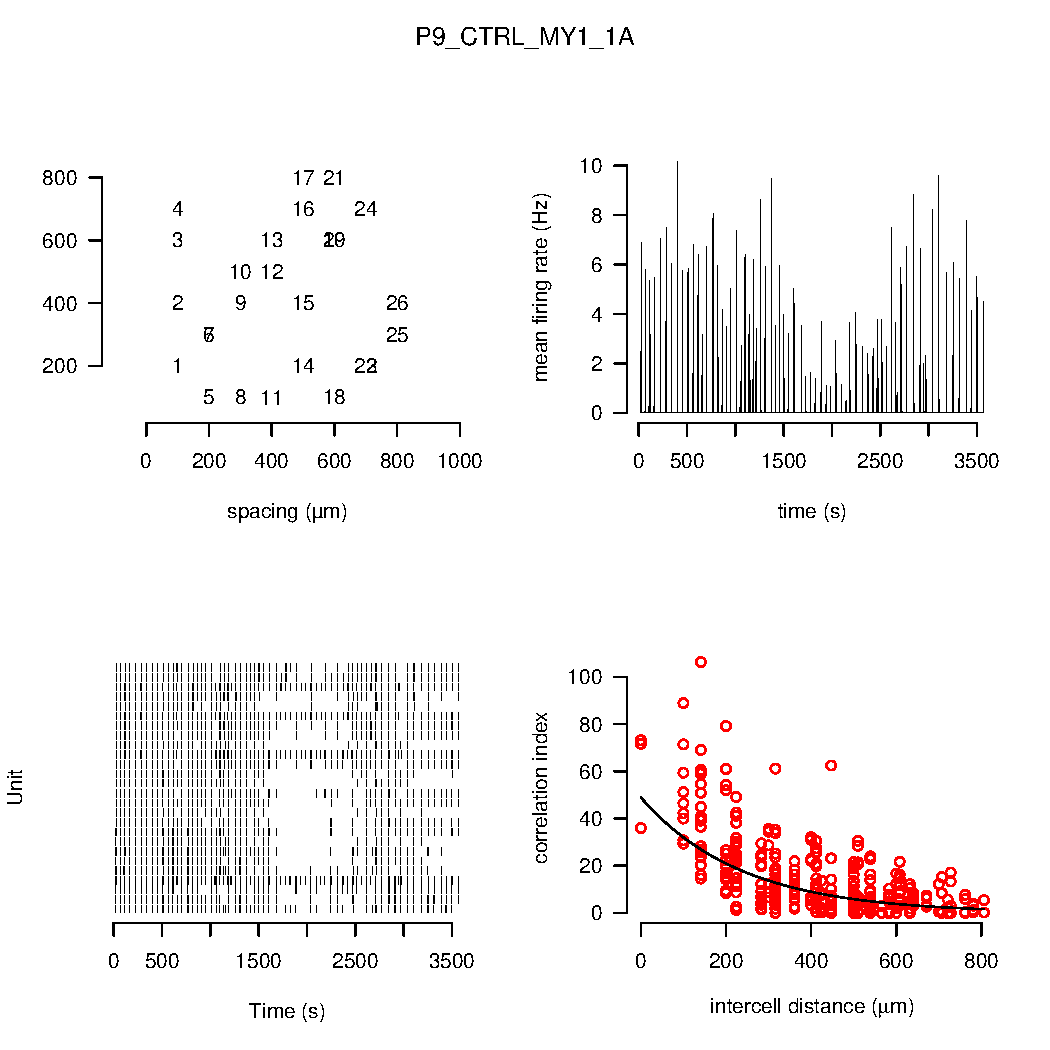
\includegraphics[width=\maxwidth]{figure/unnamed-chunk-1} 

\end{knitrout}


A convention of the program is that all data referring to a recording
is stored within an object of class \texttt{mm.s}, which is actually a
list.  So, when new data/results are collected for a recording, I tend
to add the new information into that object (e.g. see how burst
analysis results are stored).

\section*{Burst analysis}

We have several routines implemented for burst analysis:

\begin{enumerate}
\item Max Interval method, as described by Neuroexplorer \citep{neuroexplorer}
\item Poisson surprise \citep{Legendy1985}
\item Rank suprise \citep{Gourevitch2007}
\end{enumerate}

Out of these, the most tested has been the MaxInterval method.
\begin{knitrout}
\definecolor{shadecolor}{rgb}{0.969, 0.969, 0.969}\color{fgcolor}\begin{kframe}
\begin{alltt}
data.file <- \hlkwd{system.file}(\hlstr{"examples"}, \hlstr{"TC89_DIV15_A.nexTimestamps"}, package = \hlstr{"sjemea"})
s <- \hlkwd{sanger.read.spikes}(data.file)
s$allb <- \hlkwd{spikes.to.bursts.surprise}(s)
\end{alltt}
\end{kframe}
\end{knitrout}


So, for example, for electrode 2, we see the following bursts (just
taking the head as there are many of them.  We can also easily plot
the number of bursts on each electrode.

\begin{knitrout}
\definecolor{shadecolor}{rgb}{0.969, 0.969, 0.969}\color{fgcolor}\begin{kframe}
\begin{alltt}
\hlkwd{head}(s$allb[[2]])
\end{alltt}
\begin{verbatim}
##      beg len     SI    durn mean.isis
## [1,]   1  19  70.76 0.06848  0.003804
## [2,]  21  60 103.03 1.95984  0.033218
## [3,]  85  14  44.38 0.08668  0.006668
## [4,] 100  56  93.56 1.92436  0.034988
## [5,] 158   6  15.44 0.05552  0.011104
## [6,] 164  68 118.08 2.17580  0.032475
\end{verbatim}
\begin{alltt}
nbursts <- \hlkwd{sapply}(s$allb, nrow)
\hlkwd{plot}(nbursts, xlab = \hlstr{"Electrode number"}, ylab = \hlstr{"Number of bursts"}, bty = \hlstr{"n"}, 
    las = 1)
\end{alltt}
\end{kframe}
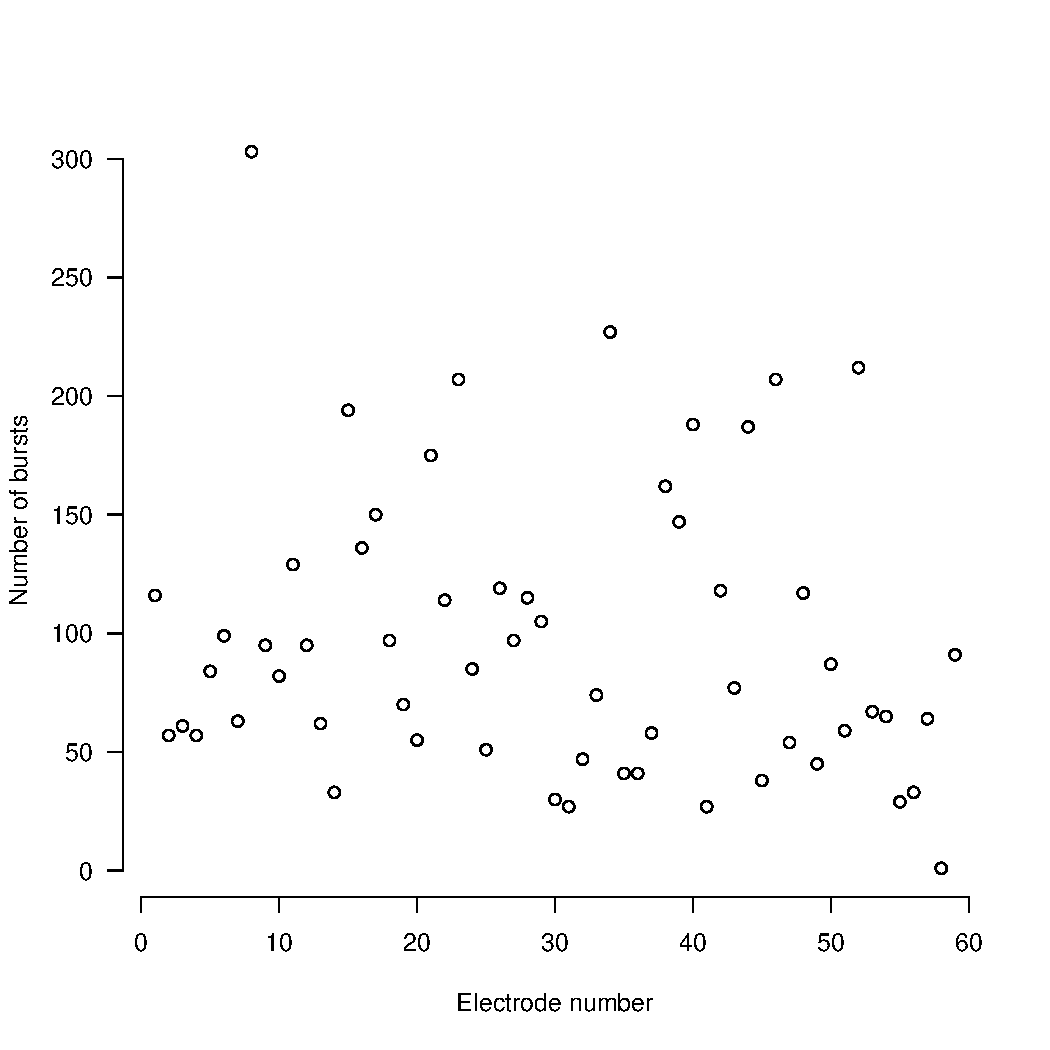
\includegraphics[width=\maxwidth]{figure/show-burst-info} 

\end{knitrout}



Once bursts are computed the resulting burst information can be
visualized on a raster assuming that the burst information is stored
in the \verb+s$allb+ component of the object.  Here we ask to see the
burst information for twenty seconds of data from just the first five trains.

\begin{knitrout}
\definecolor{shadecolor}{rgb}{0.969, 0.969, 0.969}\color{fgcolor}\begin{kframe}
\begin{alltt}
\hlkwd{plot}(s, beg = 100, end = 200, show.bursts = TRUE, whichcells = 1:5)
\end{alltt}
\end{kframe}
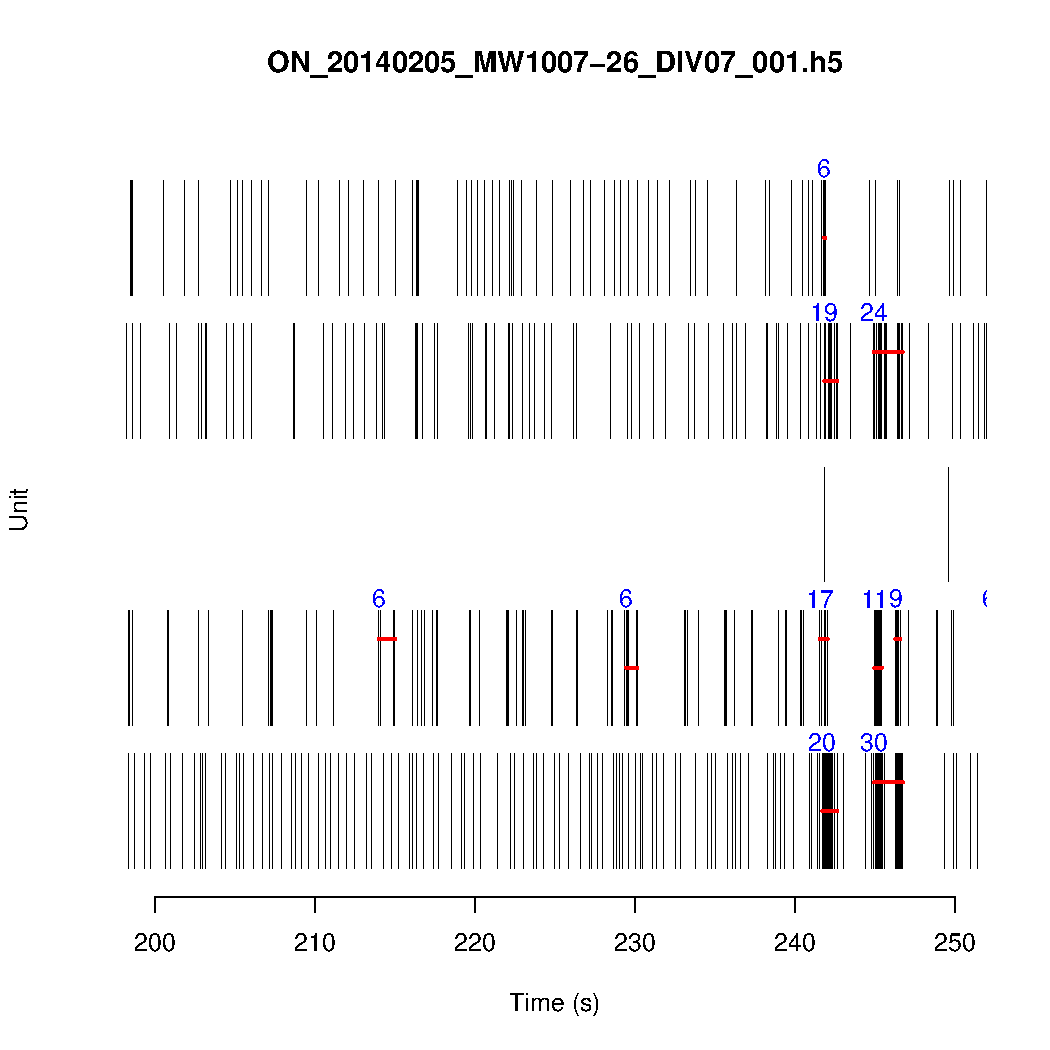
\includegraphics[width=\maxwidth]{figure/burst-raster} 

\end{knitrout}


Bursts are indicated with a red horizontal line, and the blue number
indicates the number of spikes in the burst.


Note: a Hidden-Markov Model (HMM) for burst analysis in R \citep{Tokdar2010}
is available in the following package:
\url{http://www.stat.duke.edu/~st118/Software/}.

can be used within this package, but in principle (computation time
aside as I expect an HMM to be slow) there should be no issue.  There
is also a generic ``bursts'' package:
\url{http://cran.r-project.org/web/packages/bursts/bursts.pdf}.


\subsection*{Log interspike intervals}

To help determine burst parameters, it is often helpful to look at a
histogram of the interspike interval, plotted on a log scale.  

TODO: add this code from
\url{~/proj/sangermea/pdn/logisi_condtable.R}.
\url{~/proj/sangermea/logisi/logisi_only1.R}

\section*{Network spikes}

Network spikes are periodic elevations in activity across the whole
array \citep{Eytan2006}.  The following example shows how they are computed.
In the resulting graph, the population ``firing rate'' (the number of
active electrodes here) is shown on the y axis, time (in seconds) on
the x axis.  The horizontal red line is a threshold set for the
minimum number of active electrodes to determine a ``network spike''.
The blue dots are the peak of each network spikes.

The mean network spike is also shown, averaged across all the network
spikes in the recording.

\begin{knitrout}
\definecolor{shadecolor}{rgb}{0.969, 0.969, 0.969}\color{fgcolor}\begin{kframe}
\begin{alltt}
\hlkwd{example}(compute.ns)
\end{alltt}
\begin{verbatim}
## 
## cmpt.n> data.file <- system.file("examples", "TC89_DIV15_A.nexTimestamps",
## cmpt.n+                          package = "sjemea")
## 
## cmpt.n> s <- sanger.read.spikes( data.file, beg=400, end=700)
## 
## cmpt.n> s$ns <- compute.ns(s, ns.T=0.003, ns.N=10,sur=100)
## 
## cmpt.n> plot(s$ns, ylab='Count', xlab='Time (s)')
\end{verbatim}
\end{kframe}
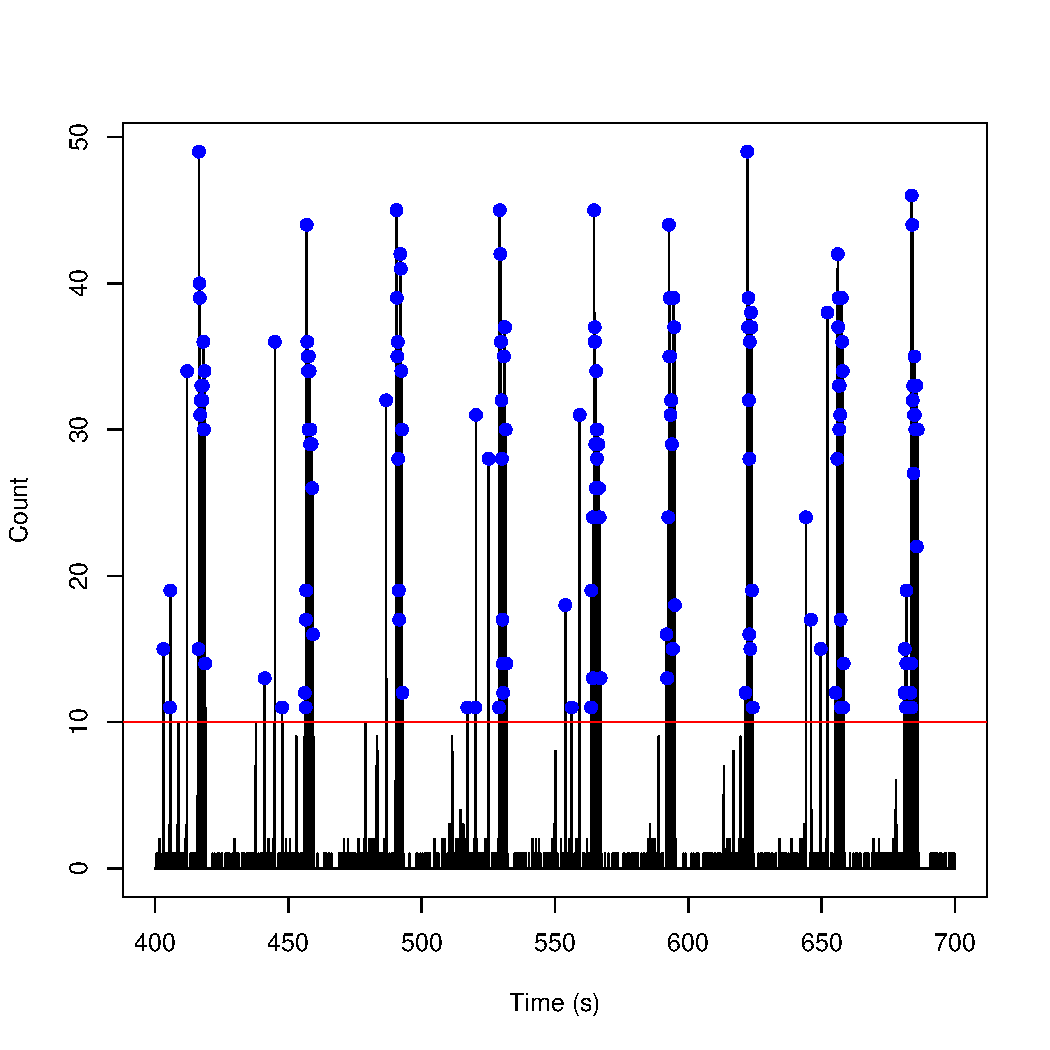
\includegraphics[width=\maxwidth]{figure/unnamed-chunk-21} 
\begin{kframe}\begin{verbatim}
## 
## cmpt.n> plot(s$ns, xlim=c(450, 500),
## cmpt.n+      xlab='Time (s)', ylab='Count')
\end{verbatim}
\end{kframe}
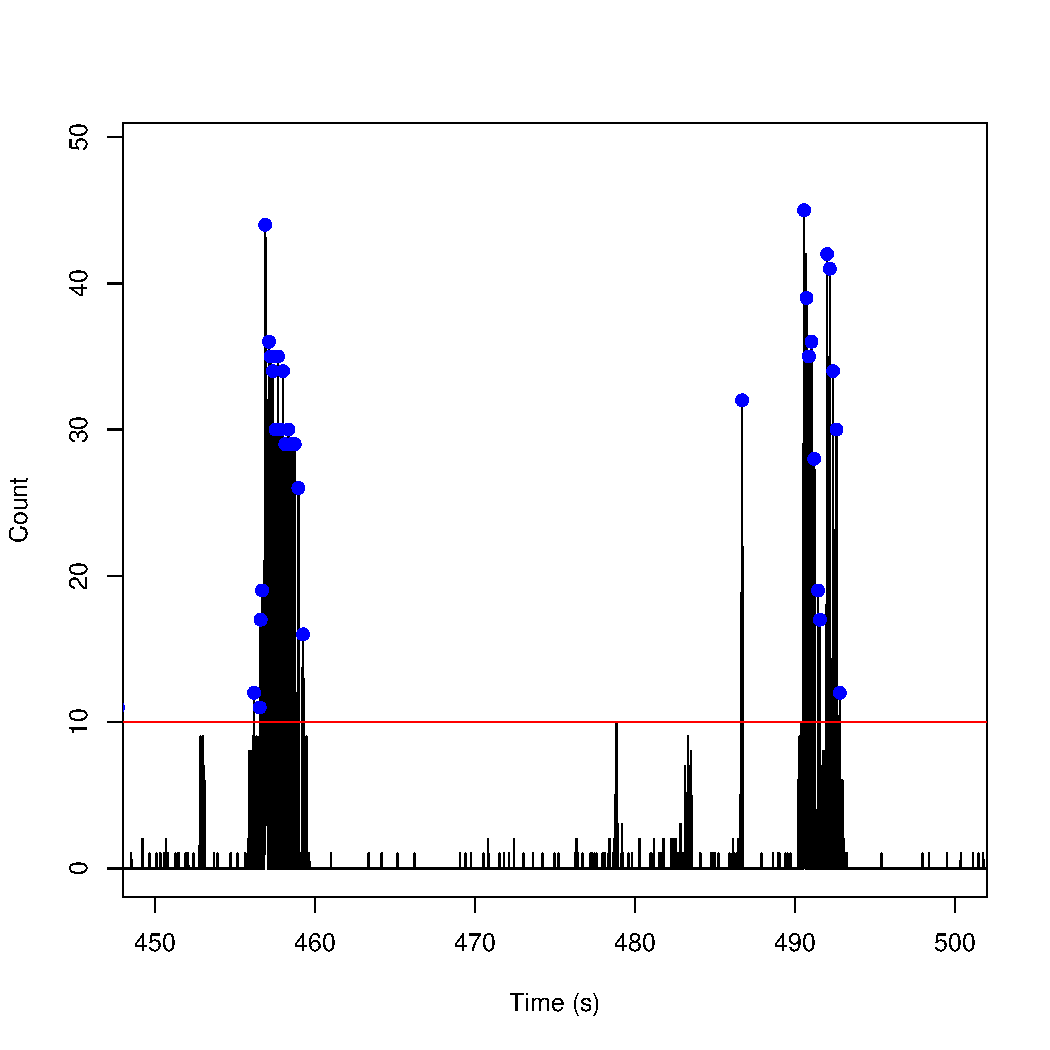
\includegraphics[width=\maxwidth]{figure/unnamed-chunk-22} 
\begin{kframe}\begin{verbatim}
## 
## cmpt.n> plot(s$ns$mean, xlab='Time (s)', ylab='Count', main='Mean NS')
\end{verbatim}
\end{kframe}
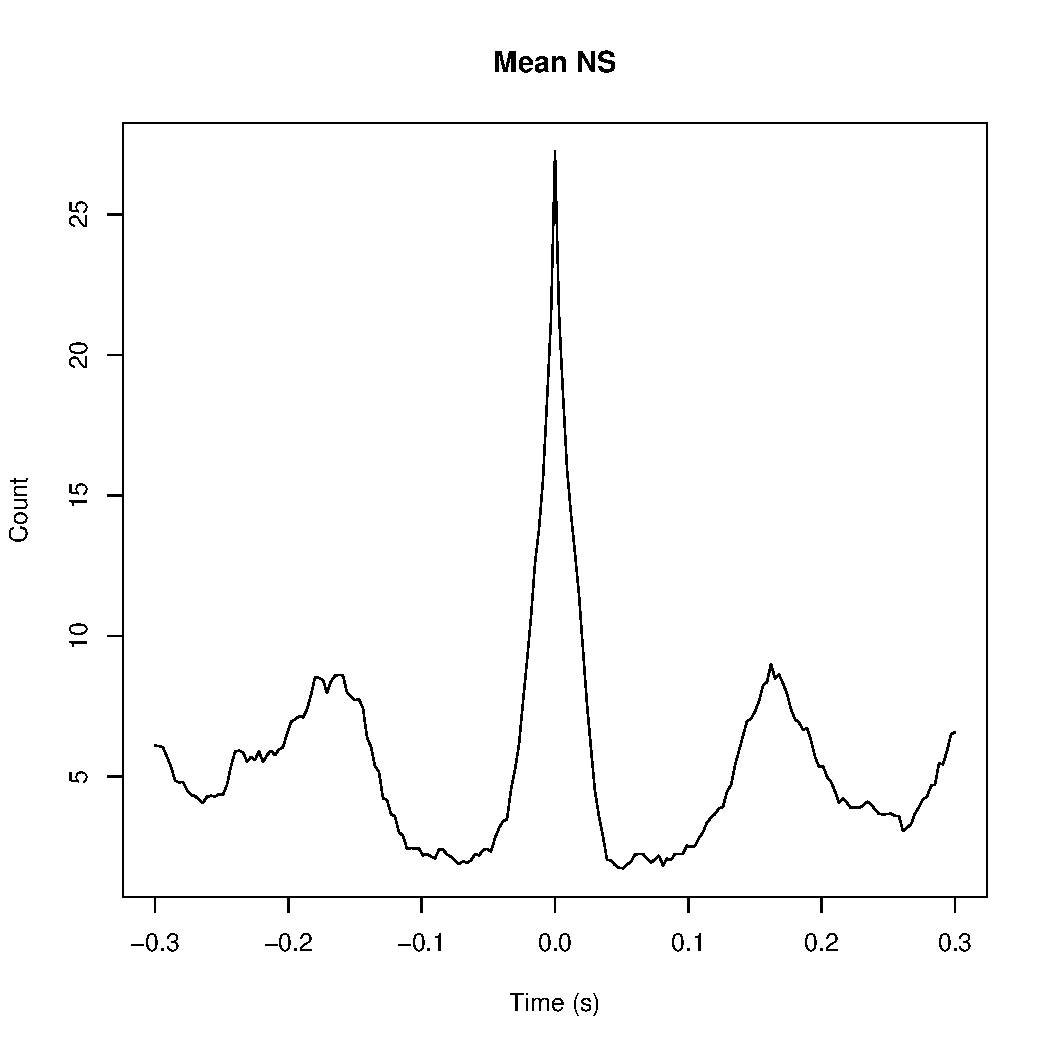
\includegraphics[width=\maxwidth]{figure/unnamed-chunk-23} 
\begin{kframe}\begin{verbatim}
## 
## cmpt.n> summary(s$ns)
## 167 network spikes
## recruitment 27.23 +/- 10.52
## FWHM 0.023 +/- 0.013 (s)
## 
## cmpt.n> s$ns$brief
##         n    peak.m   peak.sd    durn.m   durn.sd 
## 167.00000  27.23353  10.51559   0.02315   0.01264 
## 
## cmpt.n> ## show.ns(s$ns)  # This shows each network spike!  Can take a long time.
## cmpt.n> 
## cmpt.n> 
## cmpt.n>
\end{verbatim}
\end{kframe}
\end{knitrout}


\section*{Correlation index}

The correlation index plot was devised by \citet{Wong1993} as a method to
estimate how correlation between any pair of neurons on the array
depends (if at all) upon the distance separating the pair.  For
retinal waves, the correlation index usually has an
exponentially-decaying profile.  For other recordings,
(e.g. hippocampal cultures), the profile tends to be flatter.

\begin{knitrout}
\definecolor{shadecolor}{rgb}{0.969, 0.969, 0.969}\color{fgcolor}\begin{kframe}
\begin{alltt}
jay.data.file <- \hlkwd{system.file}(\hlstr{"examples"}, \hlstr{"P9_CTRL_MY1_1A.txt"}, package = \hlstr{"sjemea"})
jay.s <- \hlkwd{jay.read.spikes}(jay.data.file)
\hlkwd{plot.corr.index}(jay.s)
\end{alltt}


{\ttfamily\noindent\color{warningcolor}{\#\# Warning: removing 17 zero entries}}\end{kframe}
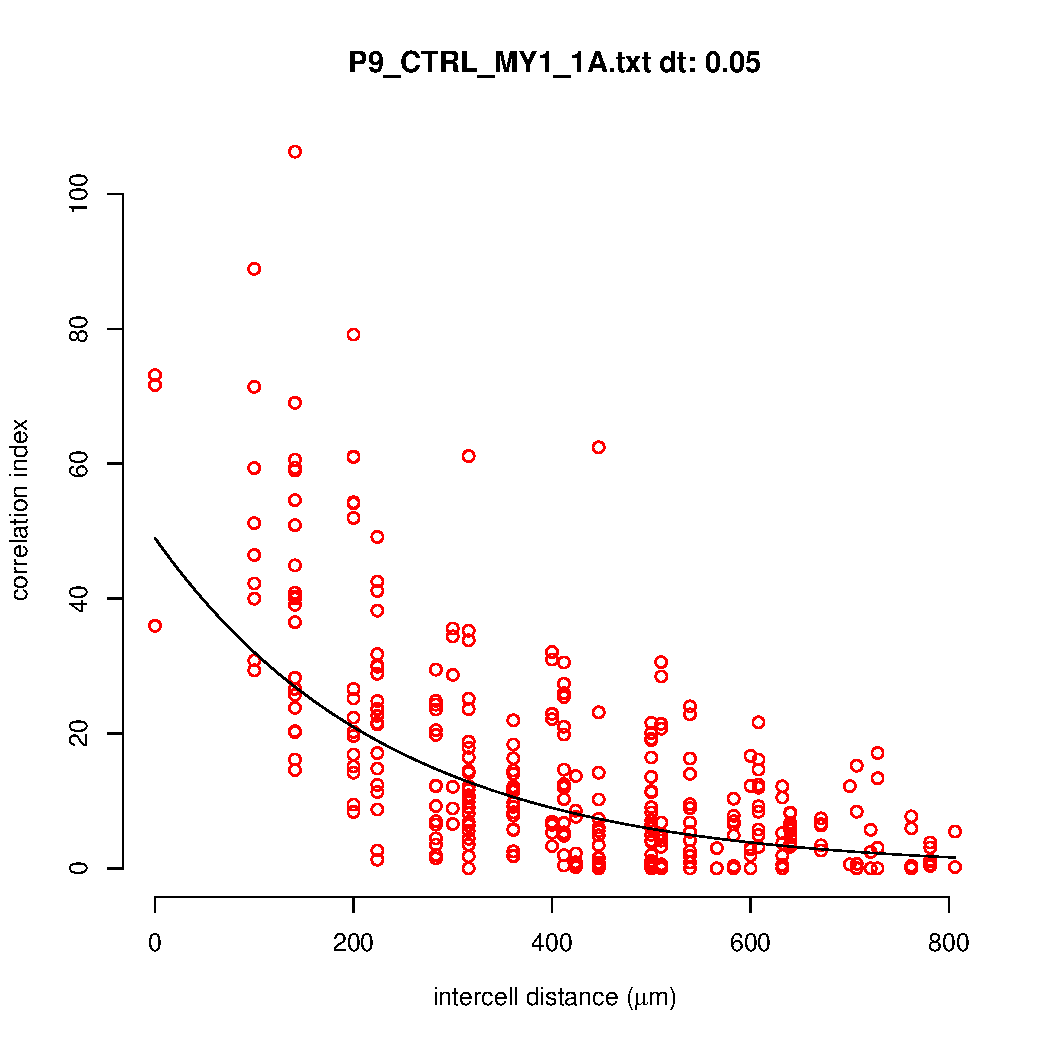
\includegraphics[width=\maxwidth]{figure/unnamed-chunk-3} 
\begin{kframe}\begin{verbatim}
## 
## Call:
## lm(formula = y.log ~ x)
## 
## Coefficients:
## (Intercept)            x  
##     3.89108     -0.00424
\end{verbatim}
\end{kframe}
\end{knitrout}


\section*{Batch analysis}

As this code is all written in the R progamming language, it scales
itself well to the notion that the analysis can be automated to run
over many data files in batch, rather than running one at a time.  To
this end, for the Genes to Cognition project, we devised a system
where data files were expected in one directory, and output files
would be written to a particular directory.  See the R function
\texttt{sanger.init} and in particular the variables
\texttt{mea.data.dir, mea.table.dir, mea.op.dir}.  A spreadsheet
containing the files to be analysed is passed to a script that
analyses each row of the spreadsheet independently.  This system was
used to analyse several hundreds of files simultaneously.


\section*{Data readers}
\label{sec:input}

The examples above have used example data stored within the package to
read in data.  Here are the names of some (not all) other readsers
that are available in the package.
 
\begin{description}
\item[ncl.read.spikes]  -- Multi-Channel system MCS output of spike
  times and cut outs.  (Named ``ncl'', as the data came from Newcastle.)
\item[jay.read.spikes] -- Used for Demas et al. (2003)  (Named ``jay''
  as the data was recorded by Jay Demas.)
\item[h5.read.spikes] -- HDF5 format, as described in the current
  ``waverepo'' project.
\item[sql.read.spikes] -- Prototype using SQL to store data.
\item[sanger.read.spikes] -- Multi-channel system from the Sanger
  Genes to Cognition project.
\item[nex.read.spikes] -- Neuroexplorer timestamp files can be read
  in.  I have adapted the matlab code from
  \url{http://www.neuroexplorer.com/code.html} to work in R.

\end{description}

\subsection*{Handling new data}

Although these old readers still work, where possible, we should use
the HDF5 format for data storage.  The preferred approach (as taken
with the ``waverepo'' project), is to convert data as soon as possible
into HDF5.

Some older routines exist for reading in binary format
(e.g. \texttt{mm.read.spikes}) but these are quite old now and
cumbersome to maintain.  Whenever possible, data collected from
laboratories should either be text or HDF5.

\subsection*{Multi-well arrays}

Through a collaboration with Dr Tim Shafer's group at EPA, we are
developing code for handling multi-well data.  (For example, so that
each well can be analysed independently in an efficient manner.)  This
introduces an extra layer of abstraction into the geometry of the
array, in that an electrode is part of a well, and there are many
wells on one array (or ``plate'').


\subsection*{Other features}

Interactive facilities for viewing spike times were in earlier
versions of the code, but Tk() widgets conflicted with the use of
parallel() code.  I think this has now been fixed, so we might be able to
return to adding interactive features.

\subsection*{History}

This package was originally written for research that was published in
\citep{Demas2003}.  Since then it has been used by several other
research groups.

\subsection*{Acknowledgements}
This work has been financially supported by grants from the Wellcome
Trust, BBSRC and EPSRC.  Zhengzheng Zhang provided the \texttt{logisi}
function.  I thank Paul Charlesworth for many discussions about
electrophysiological analysis.



\bibliographystyle{jneurosci}
\bibliography{sjemea}

\subsection*{Compiling this document}

\begin{knitrout}
\definecolor{shadecolor}{rgb}{0.969, 0.969, 0.969}\color{fgcolor}\begin{kframe}
\begin{alltt}
\hlkwd{require}(knitr)
\hlkwd{knit2pdf}(\hlstr{"sjemea-intro.Rnw"})
\end{alltt}
\end{kframe}
\end{knitrout}





\end{document}
